\chapter{Verfahrensbeschreibung}

\section{Einlesen}

Die Klasse \texttt{TextFileReader} ist für das strukturierte Einlesen und Validieren der Eingabedatei zuständig.
Sie implementiert das Interface \texttt{Reader} und liefert mit der Methode \texttt{read()} ein vollständig initialisiertes \texttt{CityDTO}-Objekt,
das alle für die Simulation notwendigen Daten kapselt.

Der Leseprozess beginnt mit einer Prüfung der Dateiexistenz sowie der korrekten UTF-8-Kodierung.
Anschließend wird die Datei zeilenweise eingelesen. Kommentare (durch \texttt{\#} eingeleitet) werden entfernt,
leere Zeilen ignoriert. Die Datei ist in drei klar strukturierte Abschnitte gegliedert:

\begin{itemize}
  \item \textbf{Zeitraum:} Enthält zwei ganzzahlige Werte:
  \begin{itemize}
    \item \texttt{maxTime} -- Die gesamte Simulationsdauer in Sekunden.
    \item \texttt{clockRate} -- Das Intervall in Sekunden, in dem der Zustand aller Fahrzeuge gespeichert wird.
  \end{itemize}
  Es wird sichergestellt, dass beide Werte gültige positive Ganzzahlen sind. Dezimalzahlen und ungültige Werte führen zu klaren Fehlermeldungen.

 

\begin{figure}[h!]
    \centering
    \caption{Zeitraum Prüfmethoden in Nassi-Shneiderman-Diagrammen dargestellt:}
    \makebox[\textwidth][c]{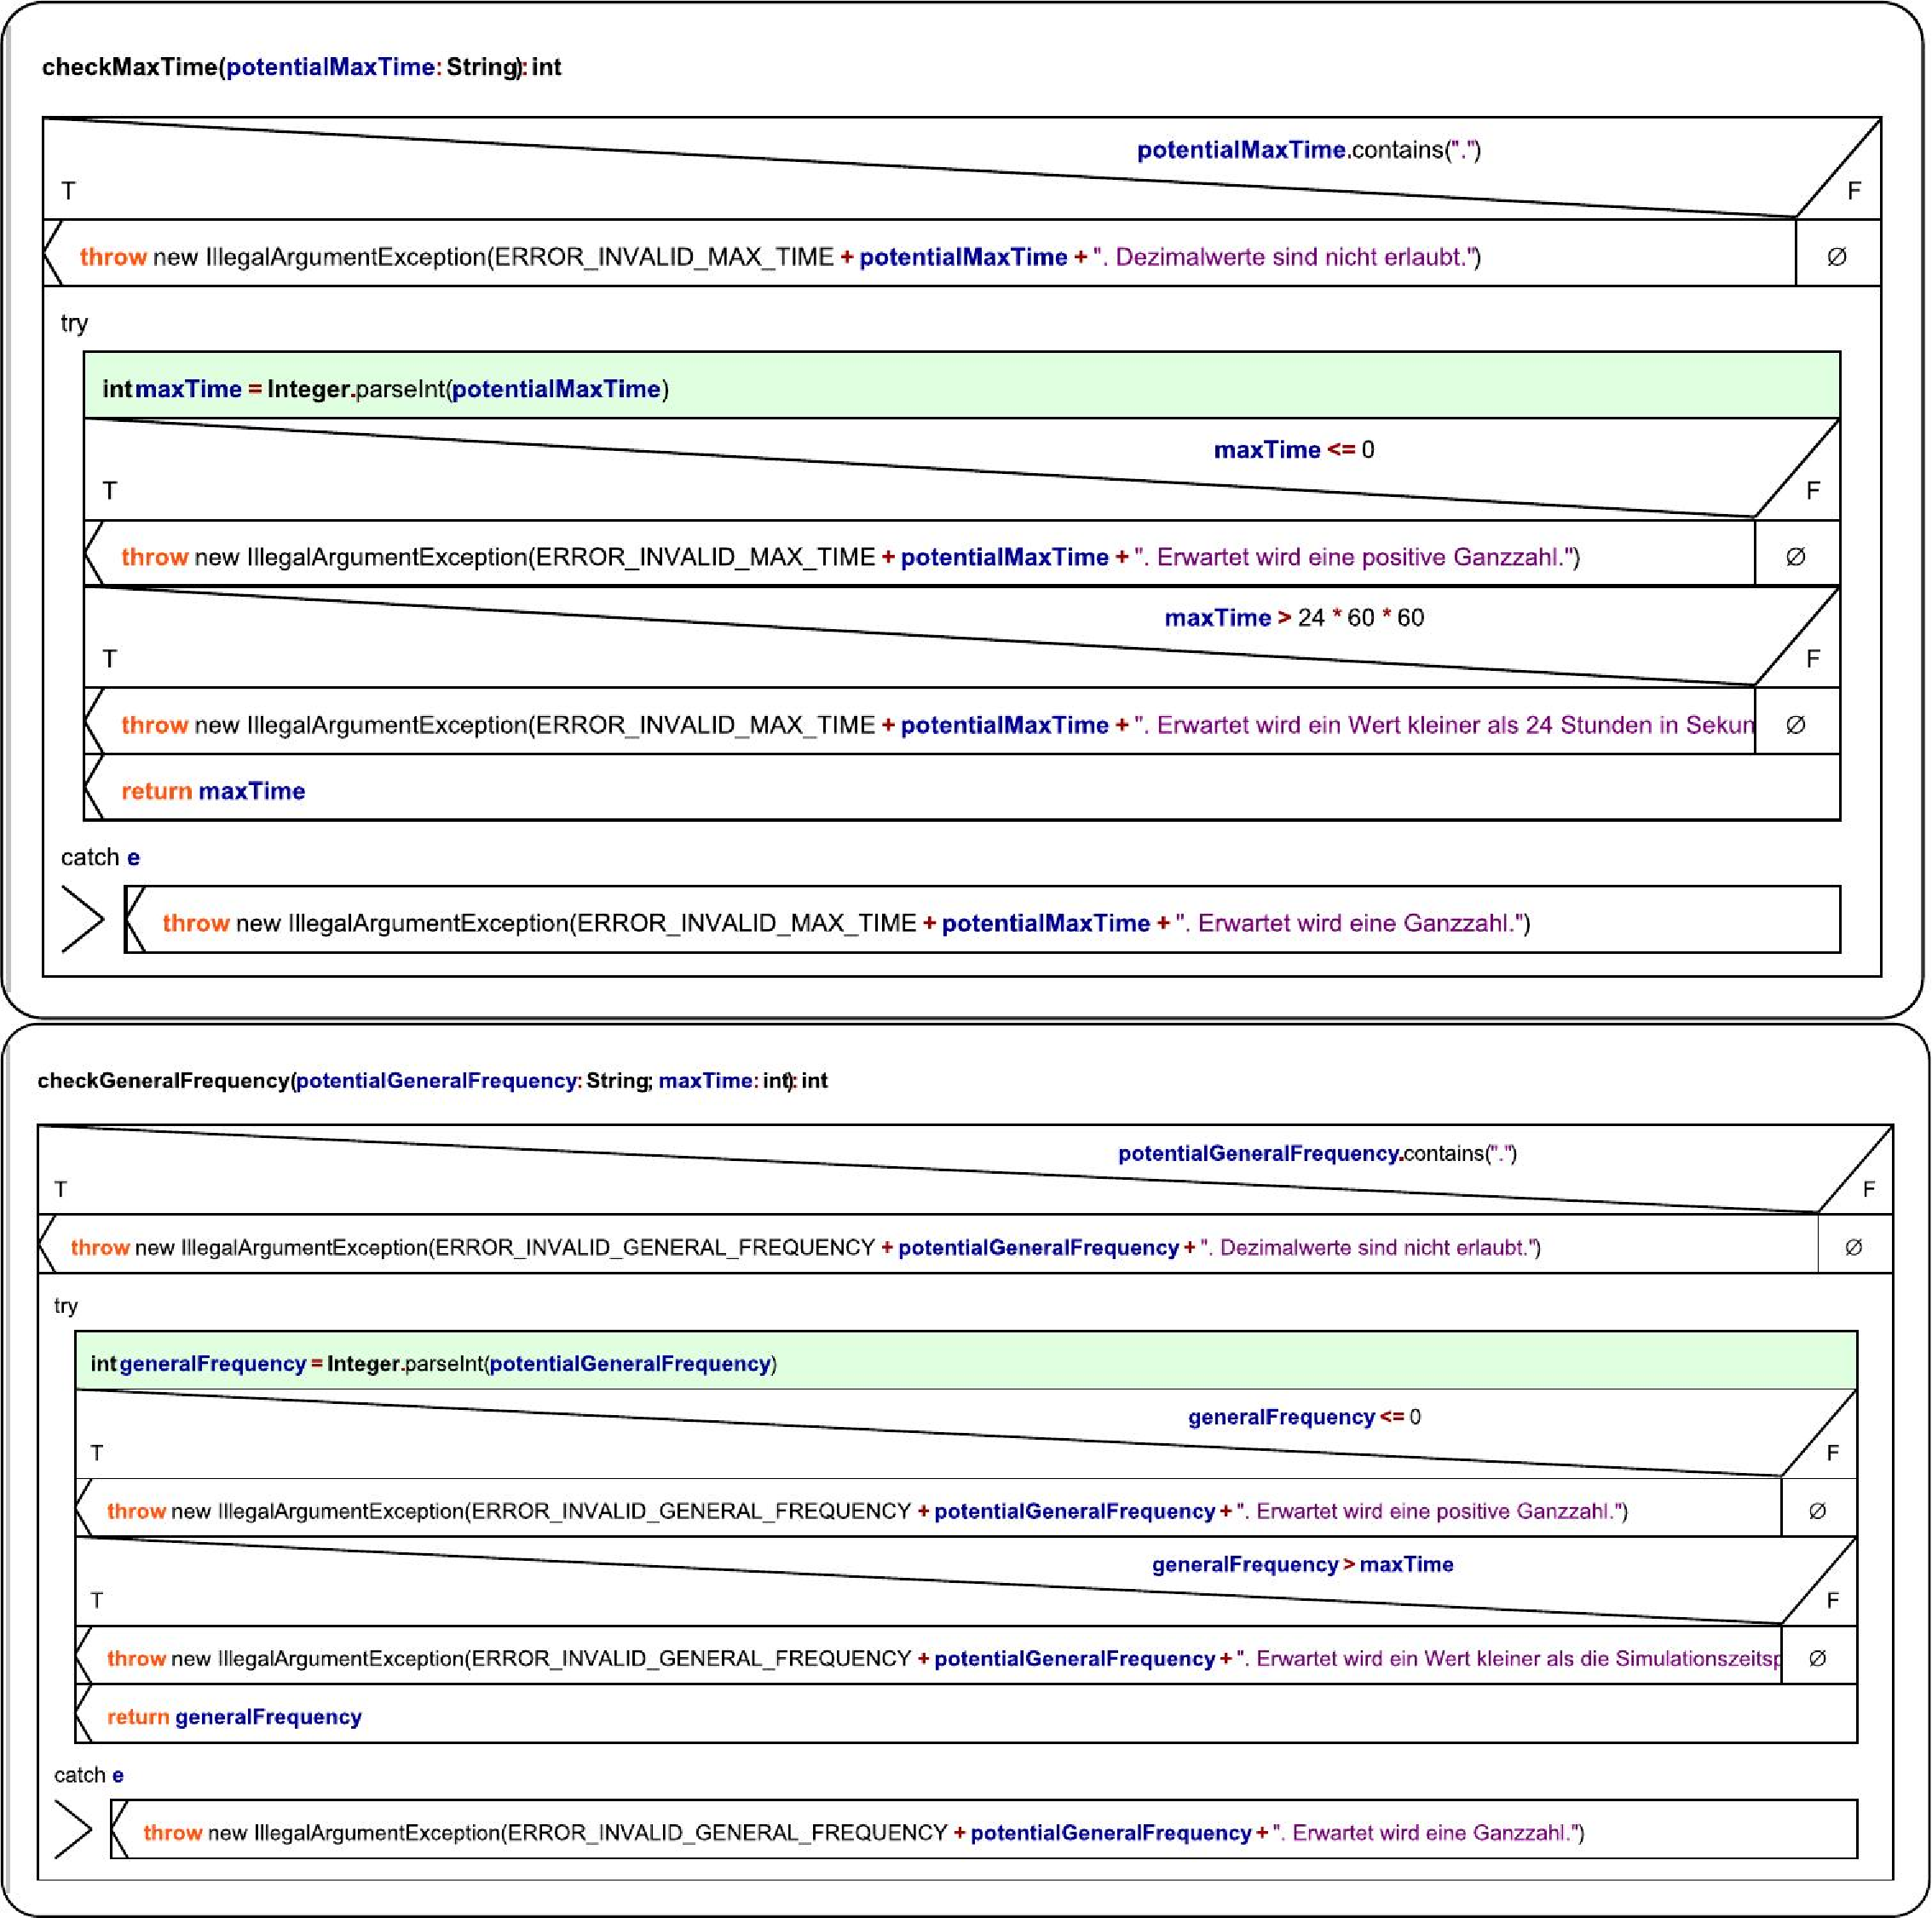
\includegraphics[width=1.3\textwidth]{nassis/TextFileReader/timeSpanChecks.pdf}}
\end{figure}

\clearpage

  \item \textbf{Einfallspunkte:} Jede Zeile beschreibt einen Einfallspunkt im Format:
  \begin{center}
    \texttt{<Name> <x> <y> <Zielkreuzung> <Frequenz>}
  \end{center}
  Dabei stehen \texttt{x} und \texttt{y} für die Koordinaten, \texttt{Zielkreuzung} für das Ziel neu erzeugter Fahrzeuge,
  und \texttt{Frequenz} für das Erzeugungsintervall.
  Es wird validiert, dass:
  \begin{itemize}
    \item jeder Name eindeutig ist,
    \item die Zielkreuzung später im Kreuzungsabschnitt existiert,
    \item Koordinaten einen Mindestabstand (0{,}1 Einheiten) zueinander einhalten,
    \item die Frequenz eine positive Ganzzahl ist.
  \end{itemize}
  Jeder gültige Eintrag wird als \texttt{EntryPoint}-Objekt gespeichert.

  Einfallspunkt Parsemethode in Nassi-Shneiderman-Diagramm (bitte reinzoomen):
  \vspace{-1.5cm} 
  \FloatBarrier
  \begin{figure}[h!]
    \vspace{-1.5cm} 
    \centering
    %\caption{Einfallspunkt Parsemethode in Nassi-Shneiderman-Diagramm:}
    \makebox[\textwidth][c]{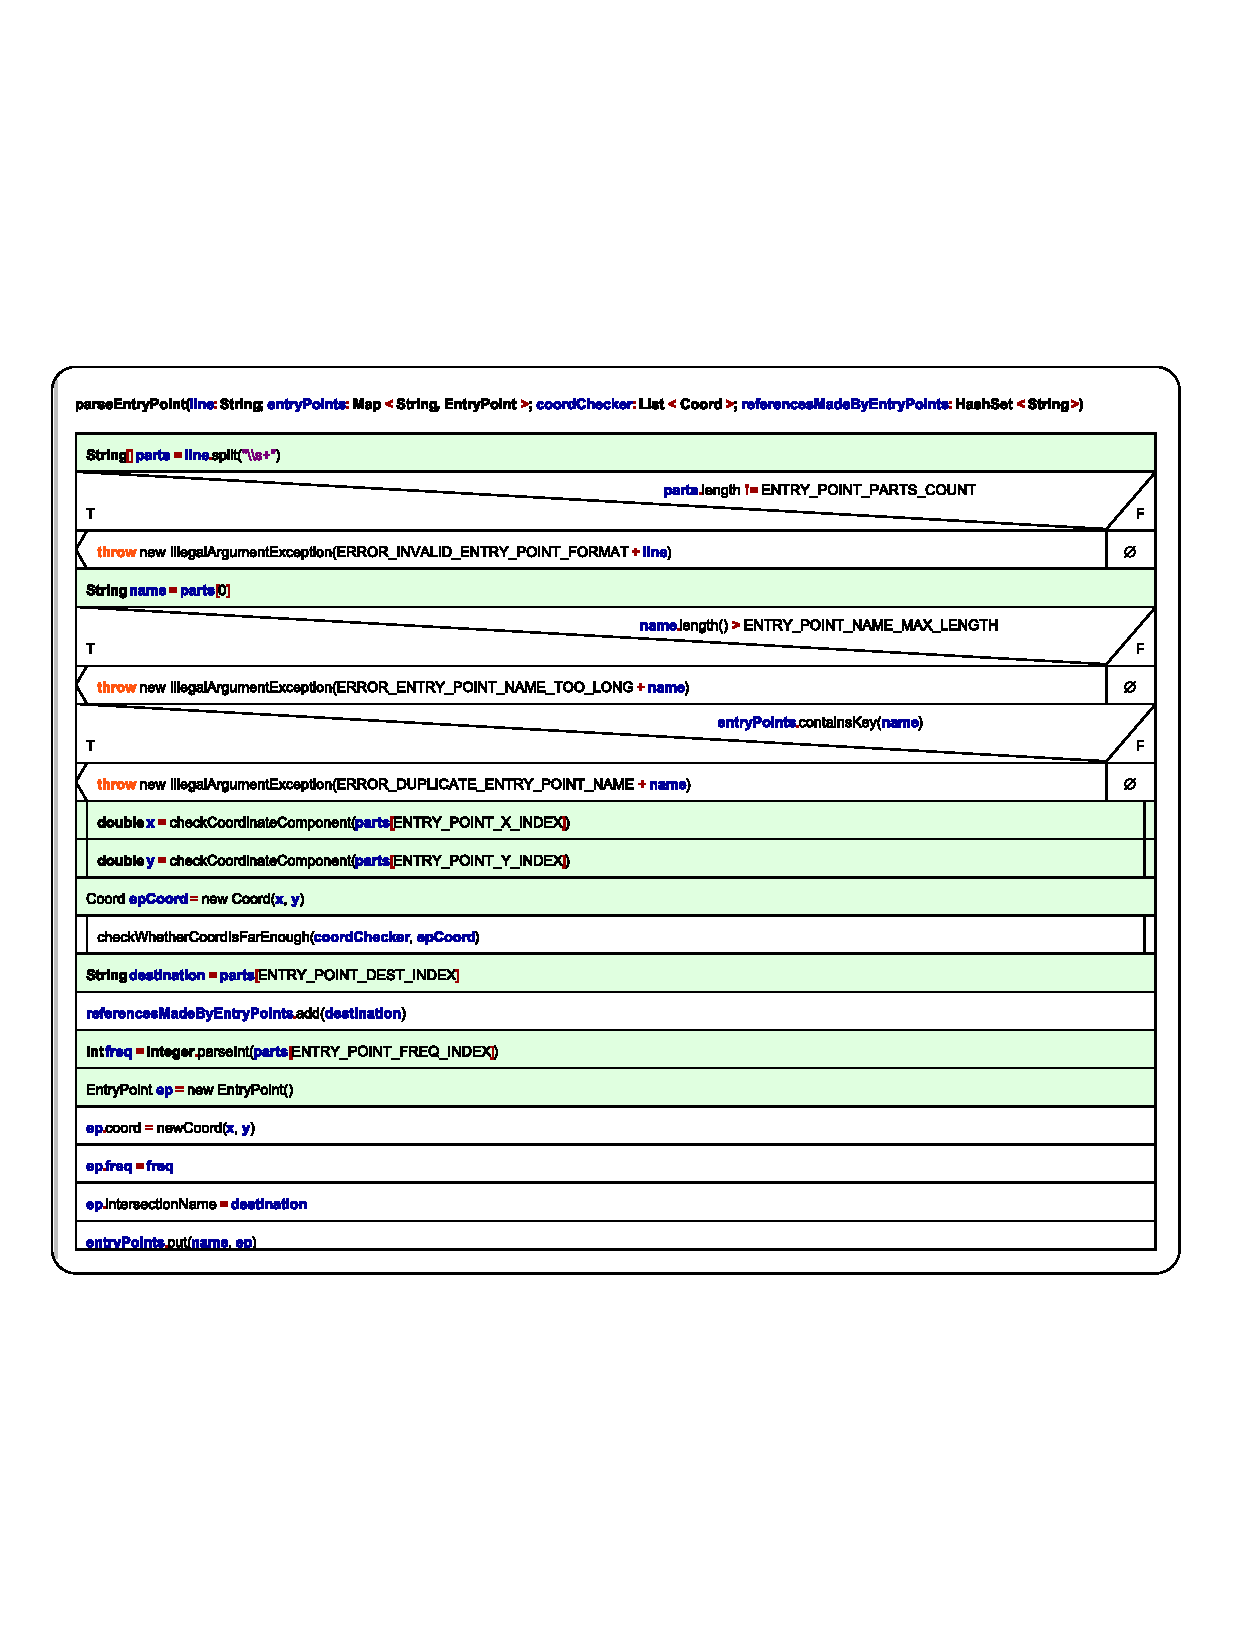
\includegraphics[width=0.9\textwidth]{nassis/TextFileReader/parseEntryPoint-4.pdf}}
\end{figure}

\clearpage

  \item \textbf{Kreuzungen:} Jede Zeile definiert eine Kreuzung und deren ausgehende Kanten:
  \begin{center}
    \texttt{<Name> <x> <y> <Ziel1> <Anteil1> <Ziel2> <Anteil2> ...}
  \end{center}
  Dabei werden:
  \begin{itemize}
    \item Koordinaten (\texttt{x}, \texttt{y}) eingelesen,
    \item Zielorte mit zugehörigen relativen Wahrscheinlichkeiten versehen,
    \item Wahrscheinlichkeiten automatisch normalisiert.
  \end{itemize}
Für jede Verbindung wird ein \texttt{DirectedEdge} (inklusive Gegenrichtung) angelegt.
Die zugehörigen statistischen Informationen werden in einem \texttt{DirectedEdgeInfo}-Objekt gespeichert.
Jede Kreuzung wird als \texttt{Intersection}-Objekt abgelegt.

Kreuzungs Parsemethode in Nassi-Shneiderman-Diagramm (bitte reinzoomen):
  \vspace{-4.5cm}
\end{itemize}
\FloatBarrier
\begin{figure}[h!]
    \vspace{-1.5cm} 
    \centering
    %\caption{Einfallspunkt Parsemethode in Nassi-Shneiderman-Diagramm:}
    \makebox[\textwidth][c]{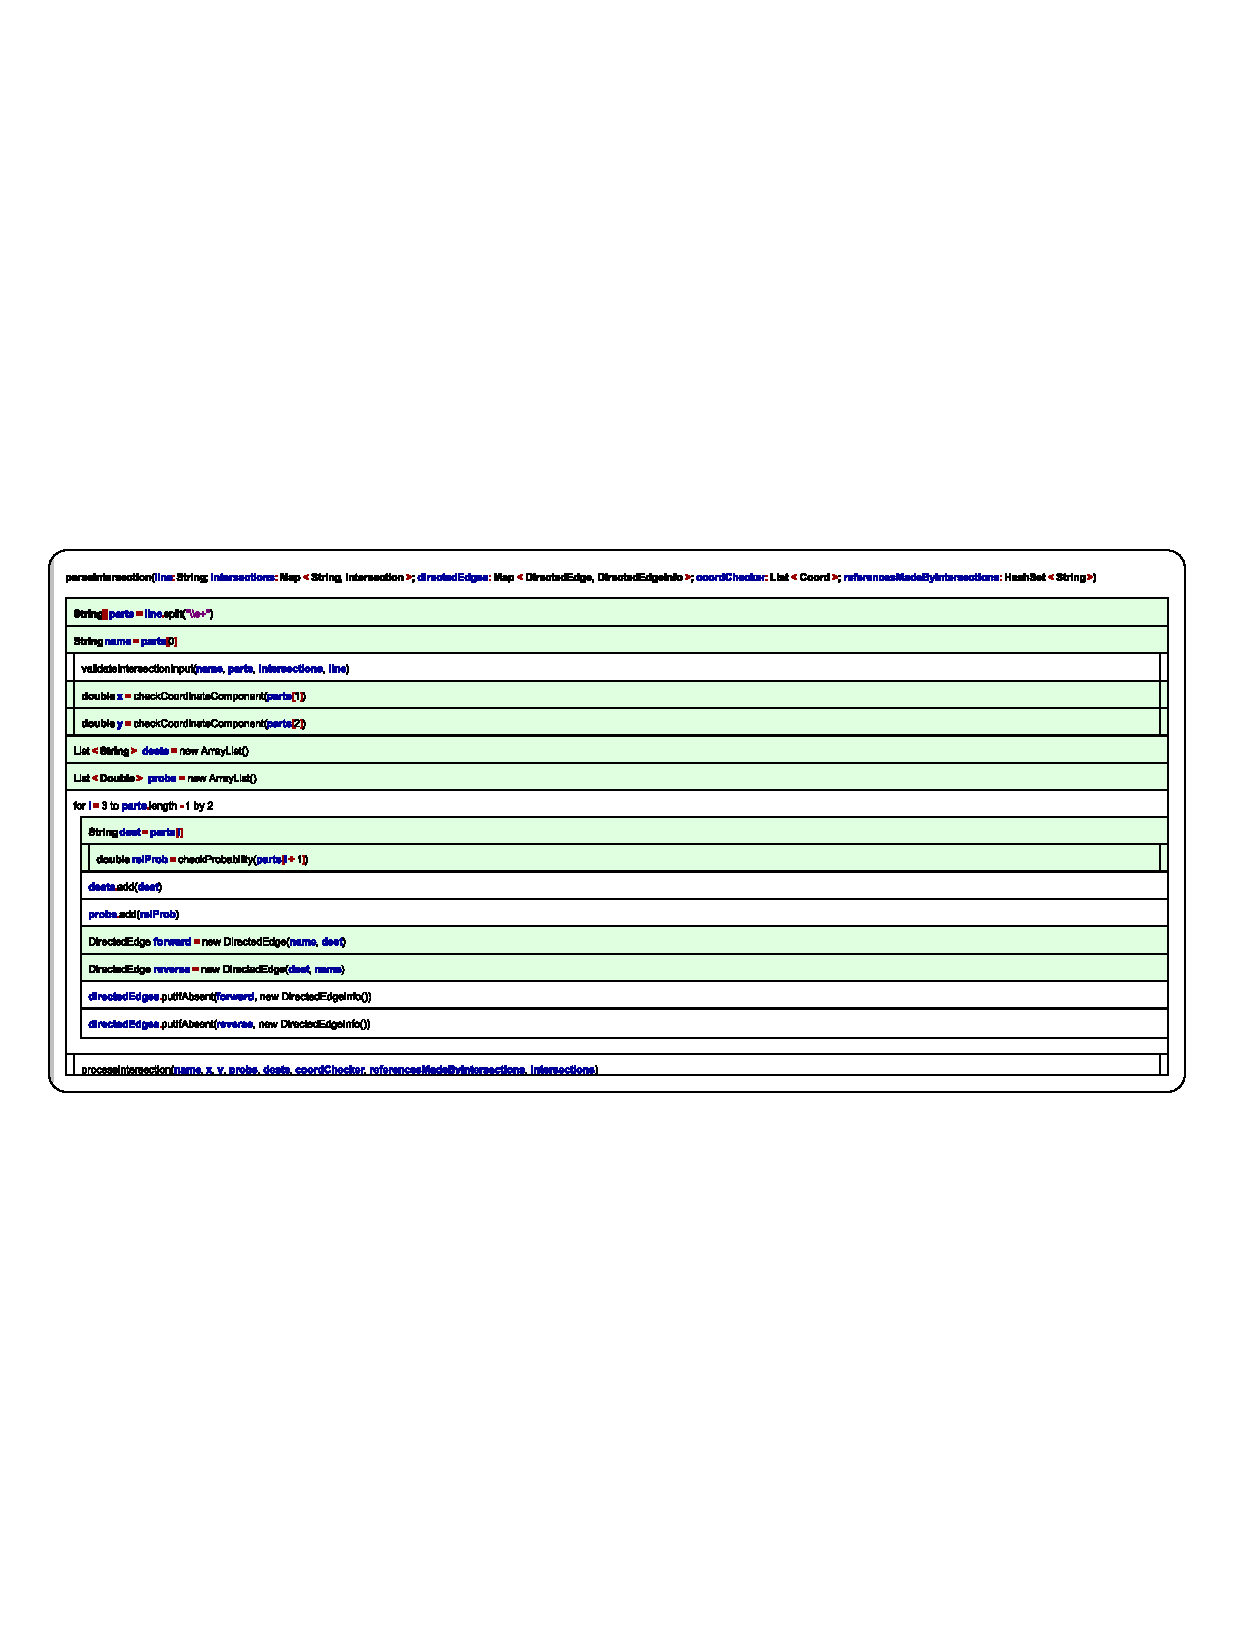
\includegraphics[width=1.11\textwidth]{nassis/TextFileReader/parseIntersection-5.pdf}}
\end{figure}

\clearpage

Nach Abschluss des Parsings werden verschiedene Konsistenzprüfungen durchgeführt:
\begin{itemize}
  \item Einfallspunkte und Kreuzungen dürfen nicht überlappen,
  \item Alle referenzierten Orte müssen existieren,
  \item Wahrscheinlichkeiten und Koordinatenwerte müssen im zulässigen Bereich liegen.
\end{itemize}

Abschließend werden alle Daten in ein \texttt{CityDTO}-Objekt überführt,
das als Grundlage für die Initialisierung der Simulation dient.

Auf der folgenden Seite lässt sich in das Nassi-Shneiderman Meisterwerk der, das \texttt{CityDTO} erzeugenden read-Methode hineinzoomen.
\clearpage
\FloatBarrier
\begin{figure}[h!]
    \vspace{-1.5cm} 
    \centering
    %\caption{Einfallspunkt Parsemethode in Nassi-Shneiderman-Diagramm:}
    \makebox[\textwidth][c]{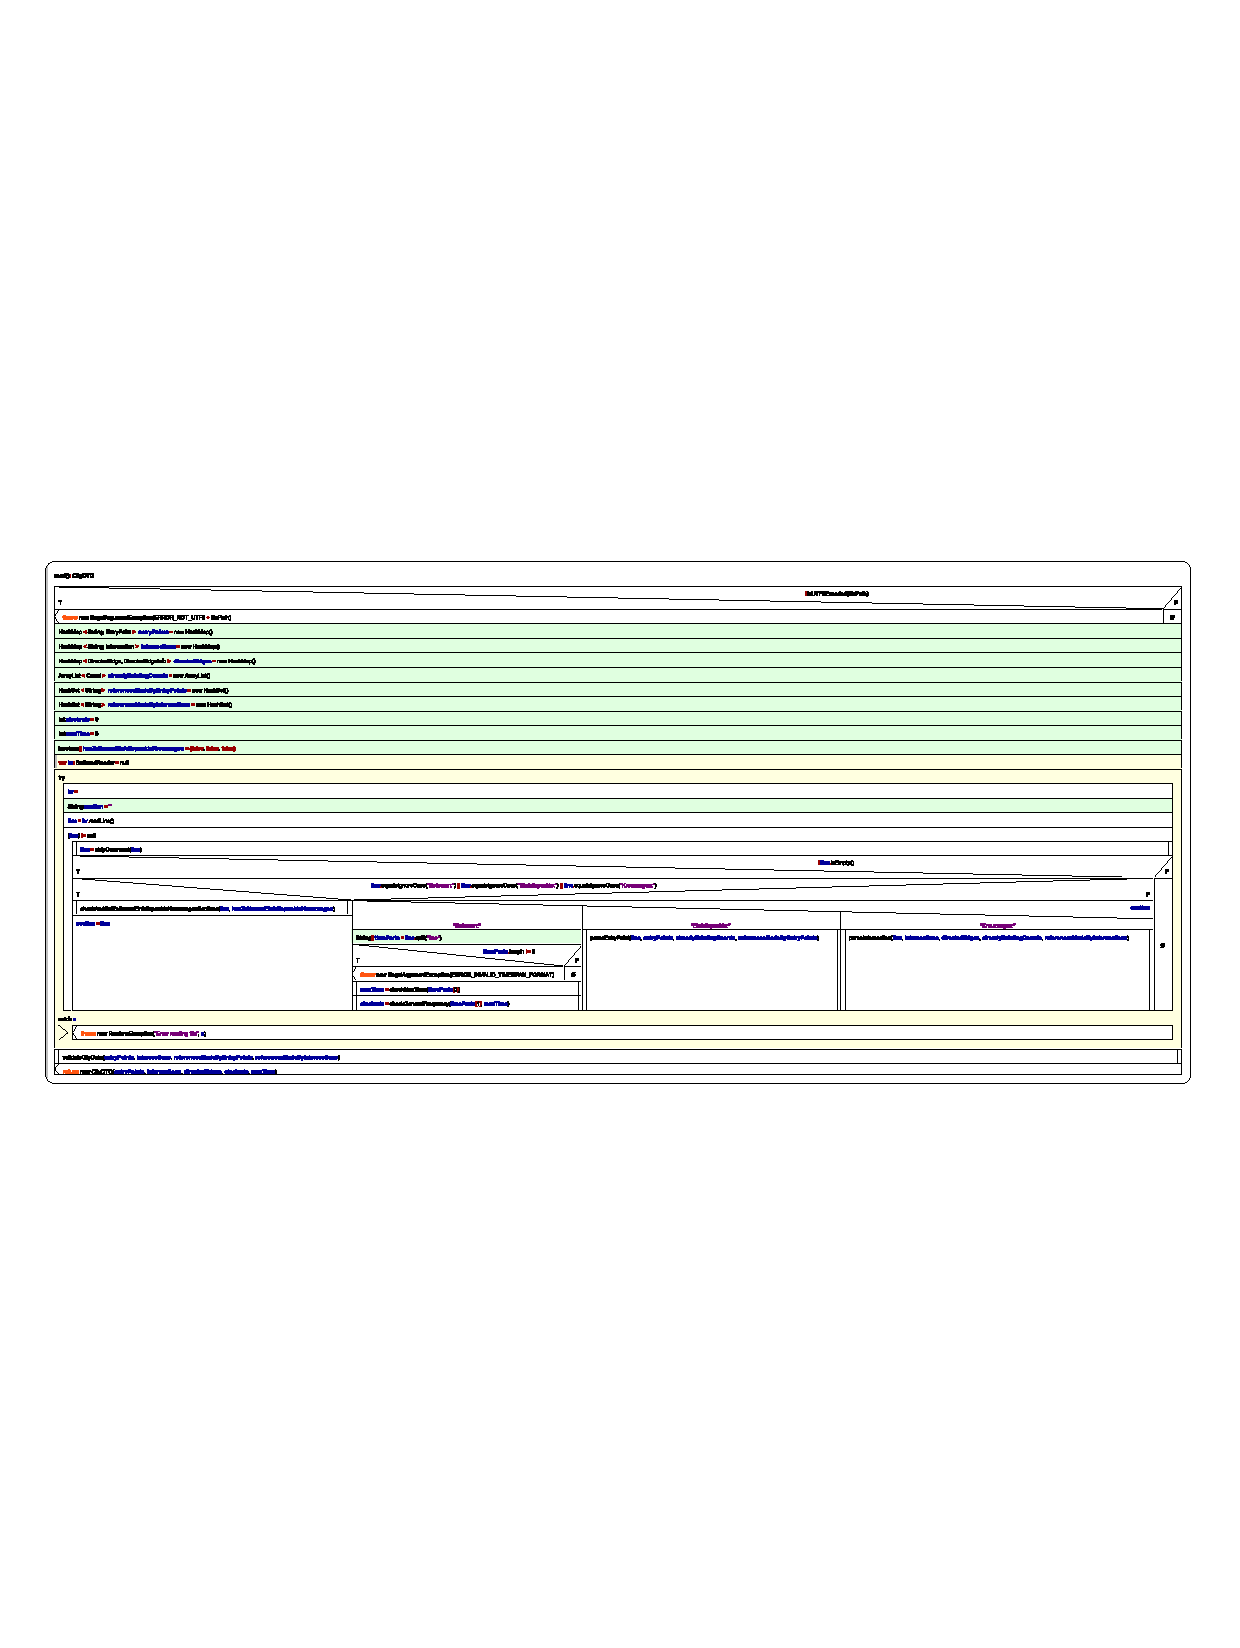
\includegraphics[width=1.5\textwidth]{nassis/TextFileReader/read-0.pdf}}
\end{figure}
\clearpage
\section{Datenhaltung}


Die Datenhaltung der Simulation erfolgt über Klassen, welche die Elemente des Verkehrsnetzes sowie den Zustand der Simulation abbilden.

\begin{itemize}
  \item \textbf{\texttt{CityDTO}}\\
  Dieses Datenübertragungsobjekt (\emph{Data Transfer Object}) bündelt alle zur Initialisierung der Simulation notwendigen Informationen:
  \begin{itemize}
    \item \texttt{entryPoints} -- Einfallspunkte als Map von Namen auf \texttt{EntryPoint}-Objekte,
    \item \texttt{intersections} -- Kreuzungen als Map von Namen auf \texttt{Intersection}-Objekte,
    \item \texttt{directedEdges} -- Gerichtete Kanten zwischen Knoten, jeweils mit zugehörigem \texttt{DirectedEdgeInfo},
    \item \texttt{clockRate} und \texttt{maxTime} -- Zeitparameter der Simulation.
  \end{itemize}

  \item \textbf{\texttt{Coord}}\\
  Diese Klasse repräsentiert zweidimensionale Koordinaten.
  Sie enthält Methoden zur Vektoroperation (Addition, Subtraktion, Normalisierung, Skalierung) sowie zur Berechnung von Distanzen.
  Die Koordinaten dienen als Grundlage für Bewegungsrichtungen und Standortspeicherungen.

  \item \textbf{\texttt{DirectedEdge}}\\
  Modelliert eine gerichtete Verbindung zwischen zwei Punkten im Verkehrsnetz.
  Zwei Felder (\texttt{from}, \texttt{to}) beschreiben die Richtung. \texttt{equals()} und \texttt{hashCode()} sind überschrieben, um die Kante als Schlüssel in HashMaps verwenden zu können.

  \item \textbf{\texttt{DirectedEdgeInfo}}\\
  Diese Klasse hält statistische Informationen zu jeder Kante:
  \begin{itemize}
    \item \texttt{totalCount} -- Gesamtanzahl aller Fahrzeuge, die die Kante jemals befahren haben,
    \item \texttt{currentNum} -- Aktuelle Anzahl an Fahrzeugen auf der Kante,
    \item \texttt{maxNum} -- Maximalanzahl an Fahrzeugen, die gleichzeitig auf der Kante waren.
  \end{itemize}
  Methoden wie \texttt{increment()}, \texttt{decrement()} und \texttt{updateMaxNum()} aktualisieren die Werte während der Simulation.

  \item \textbf{\texttt{EntryPoint}}\\
  Stellt einen Punkt dar,
  an dem Fahrzeuge ins Netz eintreten.
  Neben der Position (\texttt{coord}) enthält das Objekt den Namen der Zielkreuzung sowie die Erzeugungsfrequenz (\texttt{freq}) neuer Fahrzeuge.

  \item \textbf{\texttt{Intersection}}\\
  Repräsentiert eine Kreuzung im Verkehrsnetz.
  Enthält eine Position und ein \texttt{NamesAndProbabilities}-Objekt,
  das die möglichen Ausfahrten mit Wahrscheinlichkeiten beschreibt.
  Methoden wie \texttt{getNewDestinationByProbability()} wählen anhand eines Zufallswerts ein neues Ziel aus.

  \item \textbf{\texttt{NamesAndProbabilities}}\\
  Eine einfache Container-Klasse für Kreuzungsverbindungen. Sie enthält zwei Arrays:
  \begin{itemize}
    \item \texttt{names} -- Zielknoten,
    \item \texttt{probabilities} -- Normalisierte Übergangswahrscheinlichkeiten.
  \end{itemize}
  Diese Struktur erleichtert die Auswahl des nächsten Ziels für Fahrzeuge an Kreuzungen.
  Denn die Wahrscheinlichkeiten müssen an jeder Kreuzung normalisiert werden, da Fahrzeuge nicht in die Richtung zurückfahren können, aus der sie gekommen sind.

  \item \textbf{\texttt{Vehicle}}\\
  Diese Klasse beschreibt den Zustand eines einzelnen Fahrzeugs.
  Sie enthält Informationen zur aktuellen Position, Bewegungsrichtung, Geschwindigkeit sowie zur Herkunft und dem Ziel.
  Die \texttt{clone()}-Methode erlaubt die Erstellung tiefer Kopien zur Historisierung der Fahrzeugbewegungen.
  Geschwindigkeit und Richtung werden kontinuierlich in der simulate() Methode der City Klasse berechnet.
\end{itemize}

Das folgende Diagramm zeigt die Struktur der Datenhaltungsklassen und deren Beziehungen zueinander.
\begin{figure}[h!]
    \centering
    %\caption{Klassenstruktur der Simulation}
    \makebox[\textwidth][c]{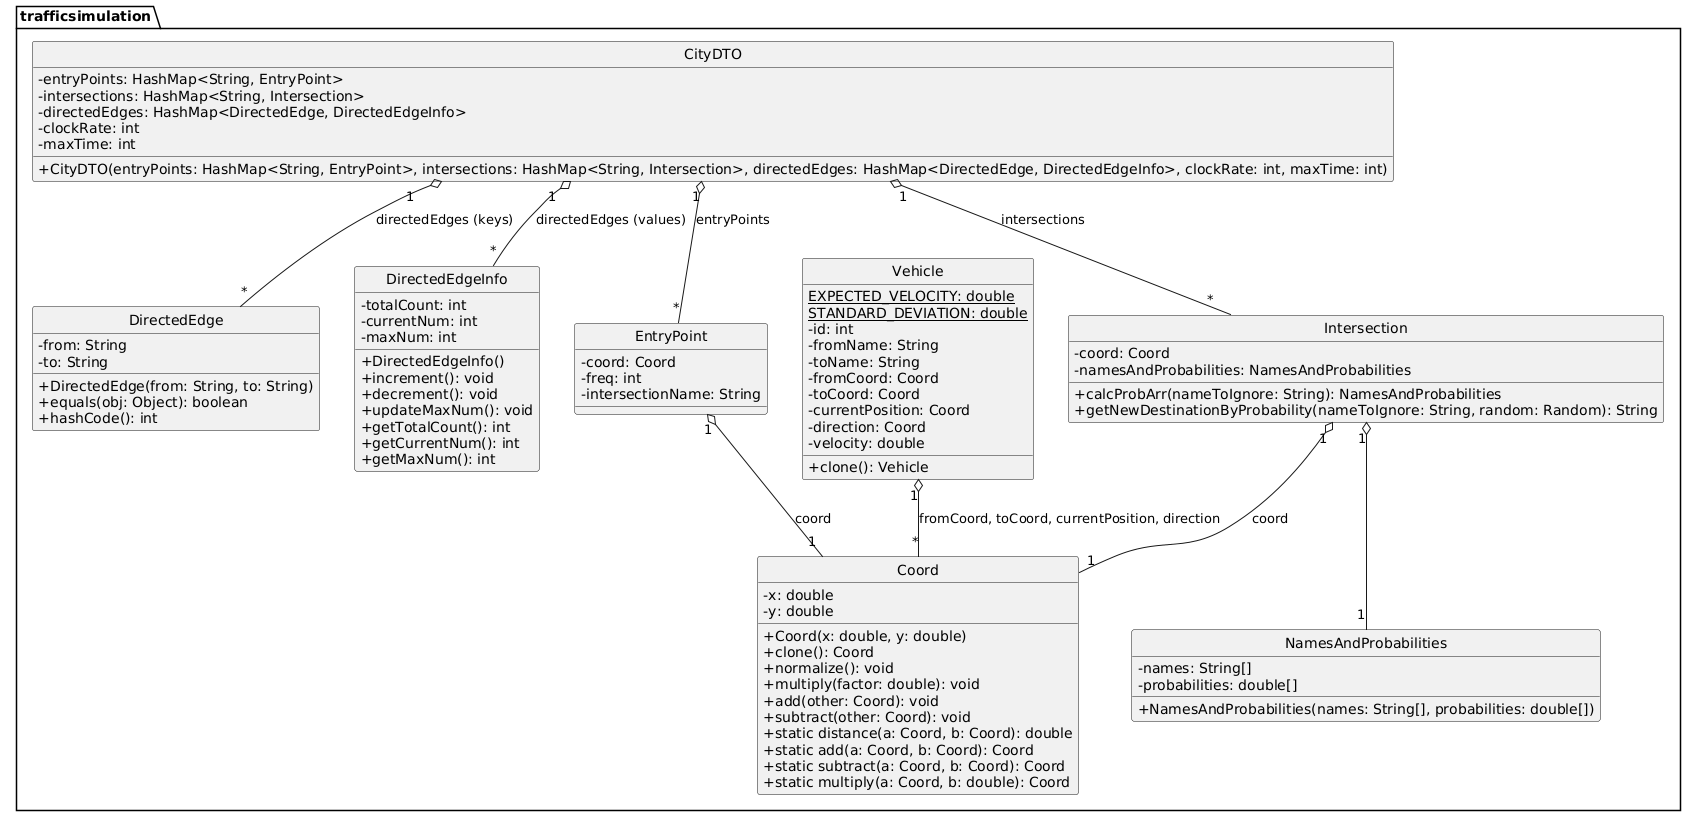
\includegraphics[width=1.3\textwidth]{umlClassDiagrams/dataHolders.png}}
\end{figure}

\clearpage

\section{Simulation}

Die Klasse City übernimmt die zentrale Steuerung der Simulation und verwaltet alle strukturellen Elemente des Straßennetzes.
Dazu zählen Einfallspunkte (EntryPoint), Kreuzungen (Intersection) sowie gerichtete Straßenverbindungen (DirectedEdge).
Neben diesen Strukturinformationen enthält die Klasse eine Liste aktuell aktiver Fahrzeuge sowie eine Historie aller Fahrzeugzustände,
die zu Analysezwecken gespeichert wird.

Der Simulationsablauf wird durch die Methode simulate() umgesetzt,
die für jeden Zeitschritt folgende Operationen durchführt:

Bewegung der Fahrzeuge: Die Methode updateVehicles() iteriert über alle aktiven Fahrzeuge und aktualisiert deren Position.
Wenn ein Fahrzeug sein Ziel erreicht hat,
wird es entweder entfernt (bei Ankunft an einem Einfallspunkt) oder ihm wird anhand der Wahrscheinlichkeiten an der aktuellen Kreuzung ein neues Ziel zugewiesen.
Dabei wird die Bewegung unter Beibehaltung der Restgeschwindigkeit auf die neue Verbindung fortgesetzt.

Fahrzeugerzeugung: Zu festgelegten Zeitintervallen (abhängig vom Taktwert des jeweiligen Einfallspunkts) wird ein neues Fahrzeug erzeugt.
Die Methode createNewVehicle() initialisiert dessen Position, Ziel, Bewegungsrichtung und zufällige Geschwindigkeit.
Außerdem wird die zugehörige Kante im Verkehrsnetz bei Fahrzeugeintritt aktualisiert.

Statistikerhebung: Nach jedem Zeitschritt wird für jede Kante im Netz die aktuelle Anzahl an Fahrzeugen geprüft und ggf. ein neuer Maximalwert gespeichert (updateDirectedEdgesMaxima()).

Aufzeichnung des Systemzustands: In Abständen, die durch den clockRate bestimmt werden,
wird der Zustand aller Fahrzeuge als tiefe Kopie in einer Historie (vehicleHistory) gespeichert.
Diese erlaubt eine spätere zeitbasierte Rekonstruktion der Fahrzeugbewegungen.

Das folgende Klassen-Diagramm zeigt die Struktur der City-Klasse und die nachfolgenden Nassi-Shneiderman-Diagramme verdeutlichen die oben beschriebene Funktionsweise.

\begin{figure}[h!]
    \centering
    \makebox[\textwidth][c]{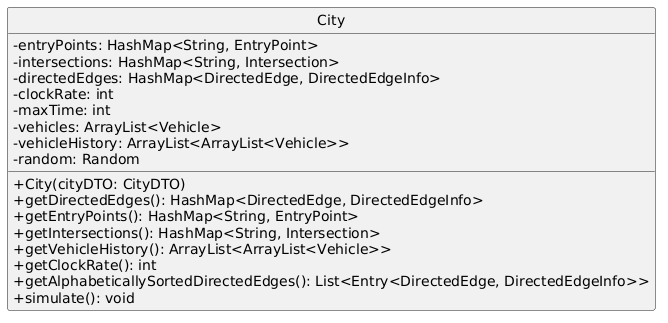
\includegraphics[width=1.3\textwidth]{umlClassDiagrams/cityBasicUmlClassDiagram.png}}
\end{figure}

\begin{figure}[h!]
    \centering
    \makebox[\textwidth][c]{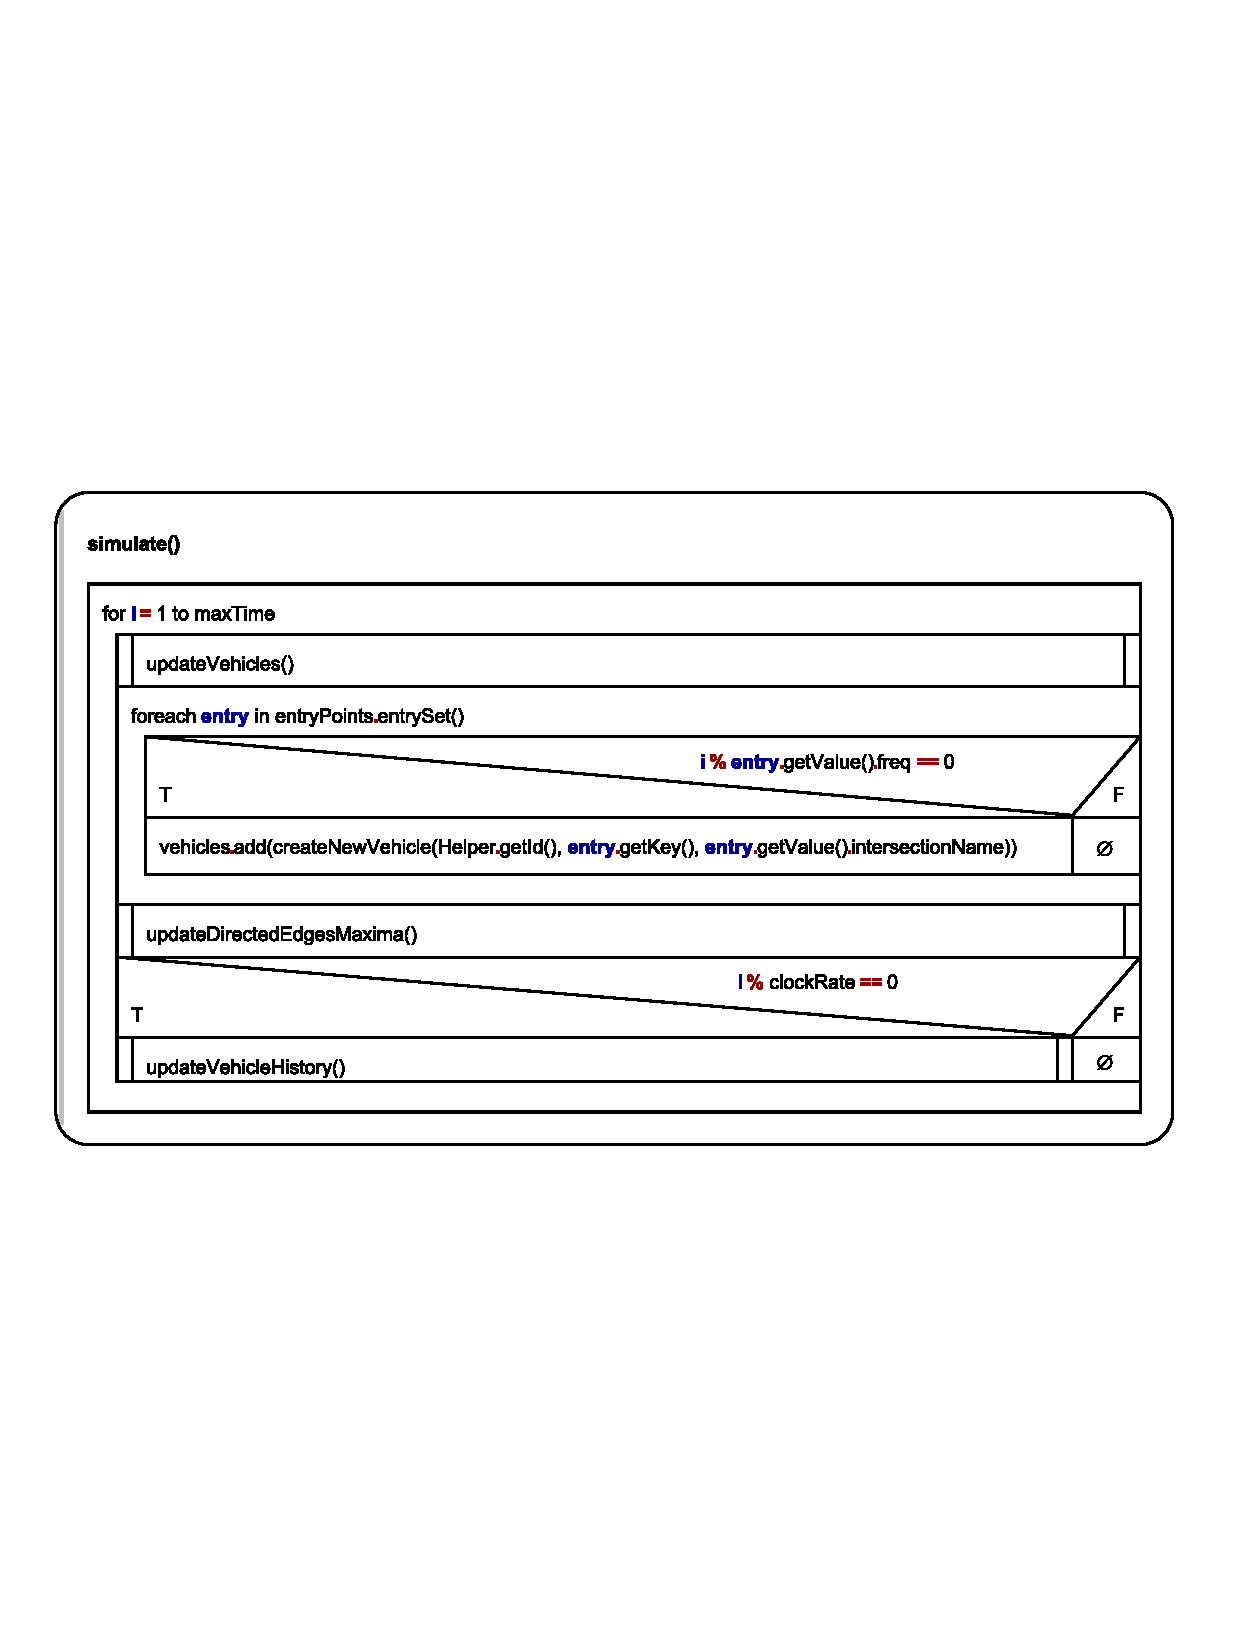
\includegraphics[width=1.3\textwidth]{nassis/City/simulate-0.pdf}}
\end{figure}

\begin{figure}[h!]
    \centering
    \makebox[\textwidth][c]{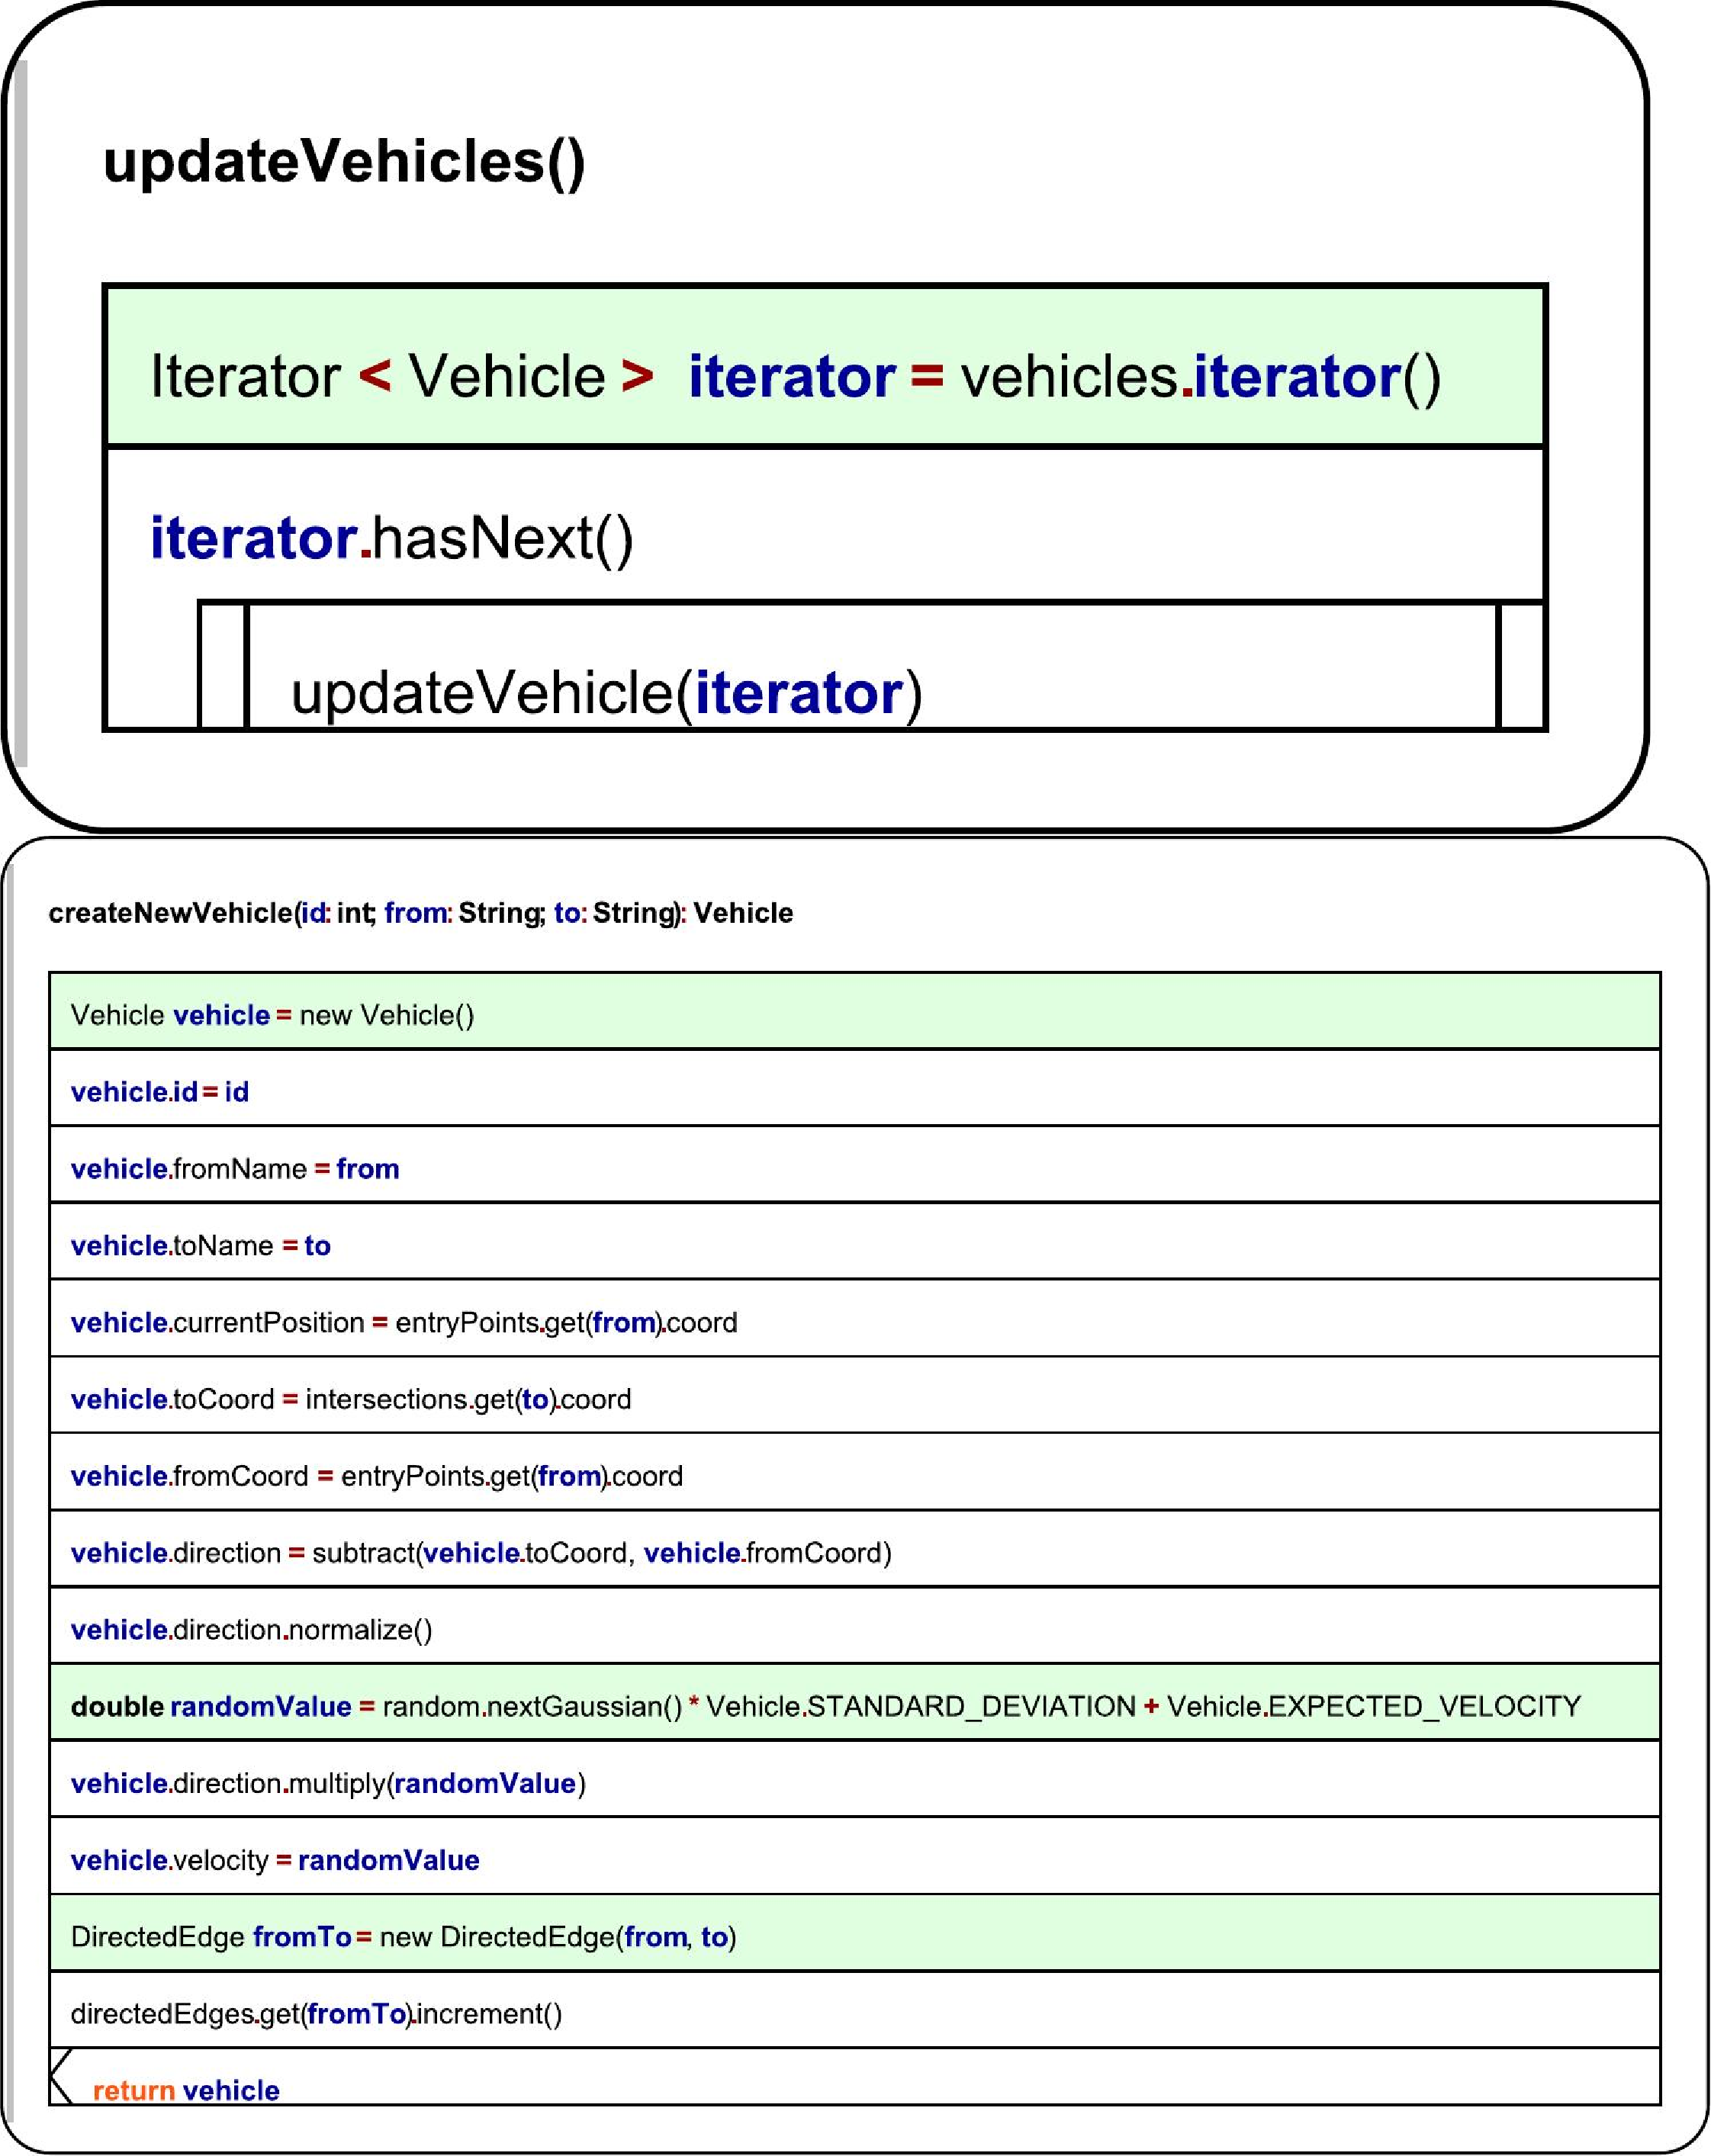
\includegraphics[width=1.3\textwidth]{nassis/City/updateVehiclesAndCreateNewVehiclesCombined.pdf}}
\end{figure}


\begin{figure}[h!]
    \centering
    \makebox[\textwidth][c]{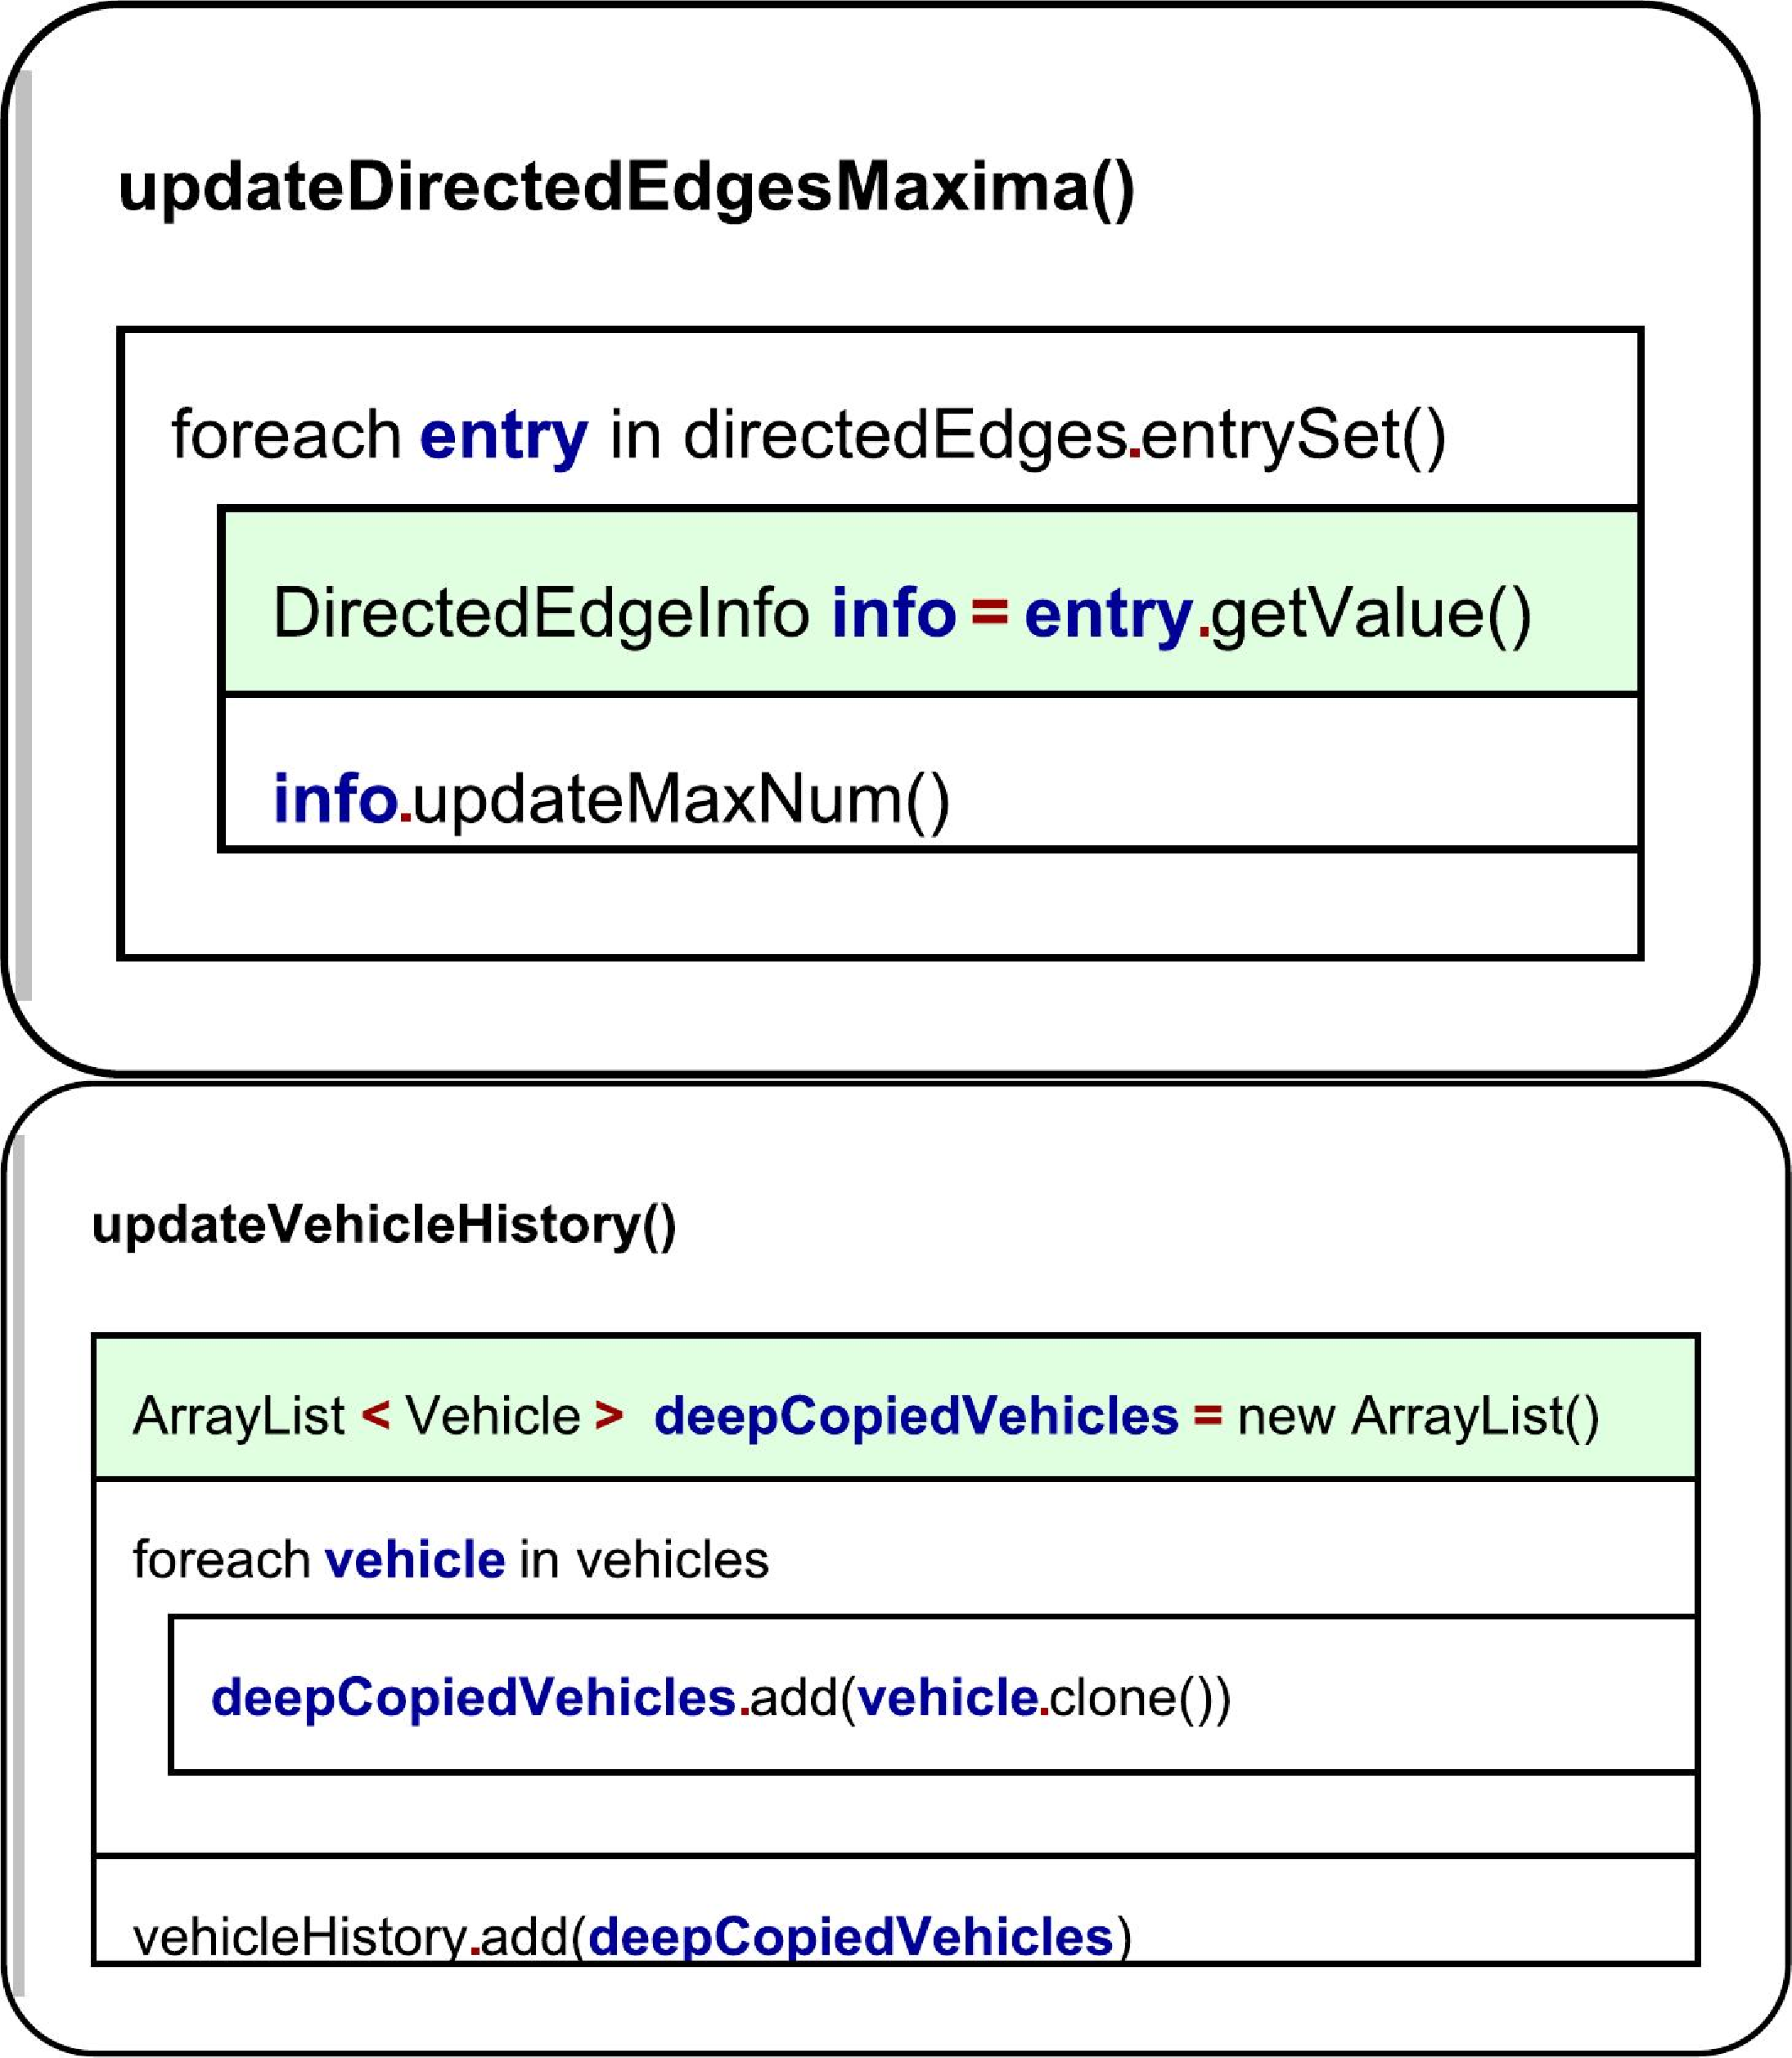
\includegraphics[width=1.3\textwidth]{nassis/City/updateMaximaAndHistory.pdf}}
\end{figure}


Darüber hinaus stellt die Klasse Funktionen zur Verfügung,
um alle gerichteten Kanten alphabetisch sortiert auszulesen (getAlphabeticallySortedDirectedEdges()),
was für die strukturierte Ausgabe der Ergebnisse genutzt wird.

\cleardoublepage

\section{Ausgabe}

Nach Abschluss der Simulation werden die Ergebnisse in drei getrennte Ausgabedateien geschrieben.

\begin{itemize}
  \item \textbf{\texttt{Plan.txt} (Klasse \texttt{PlanWriter})} \\
  Diese Datei enthält alle gerichteten Straßenverbindungen als Koordinatenpaare:
  \begin{center}
    \texttt{x1 y1 x2 y2}
  \end{center}
  wobei \texttt{x1 y1} die Start- und \texttt{x2 y2} die Zielposition einer Kante angeben. Die Ausgabe erfolgt alphabetisch sortiert nach Start- und Zielnamen.

  \FloatBarrier
    \vspace{-2cm} 
\begin{figure}[h!]
    \vspace{-2cm} 
    \centering
    \makebox[\textwidth][c]{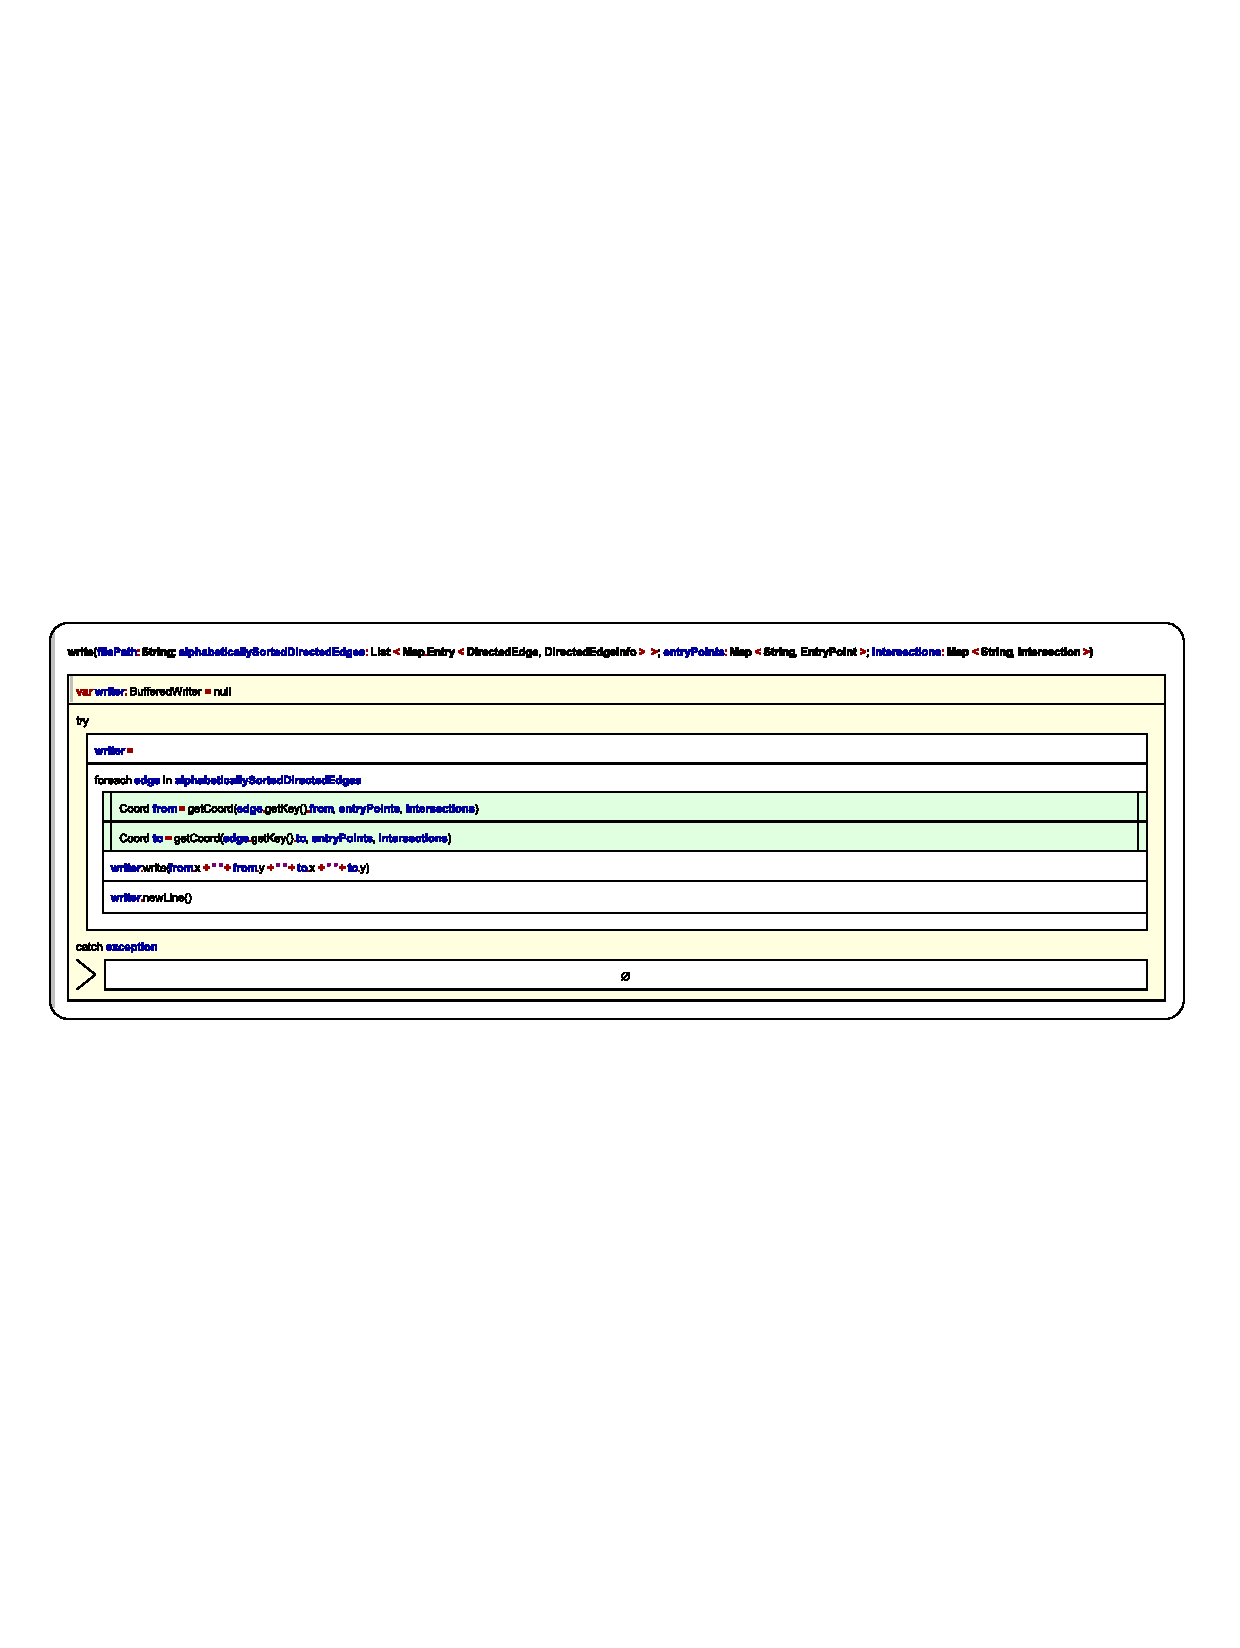
\includegraphics[width=1.05\textwidth]{nassis/Output/write-4.pdf}}
\end{figure}

\clearpage

  \item \textbf{\texttt{Statistik.txt} (Klasse \texttt{StatisticWriter})} \\
  Für jede Kante werden zwei Werte normiert auf 100 Meter Straßenlänge berechnet und ausgegeben:
  \begin{itemize}
    \item \textbf{Gesamtanzahl Fahrzeuge:} Wie viele Fahrzeuge die Kante insgesamt passiert haben.
    \item \textbf{Maximale Anzahl Fahrzeuge:} Die maximale Anzahl gleichzeitig auf der Kante befindlicher Fahrzeuge während der Simulation.
  \end{itemize}
  Beide Werte werden berechnet, indem die Rohwerte durch die euklidische Länge der jeweiligen Kante geteilt werden, wobei die Berechnung auf 100 Meter normiert ist.
  Die Ausgabe erfolgt ebenfalls alphabetisch sortiert nach Start- und Zielnamen.

  \FloatBarrier
      \vspace{-2cm} 
\begin{figure}[h!]
        \vspace{-2cm} 
    \centering
    \makebox[\textwidth][c]{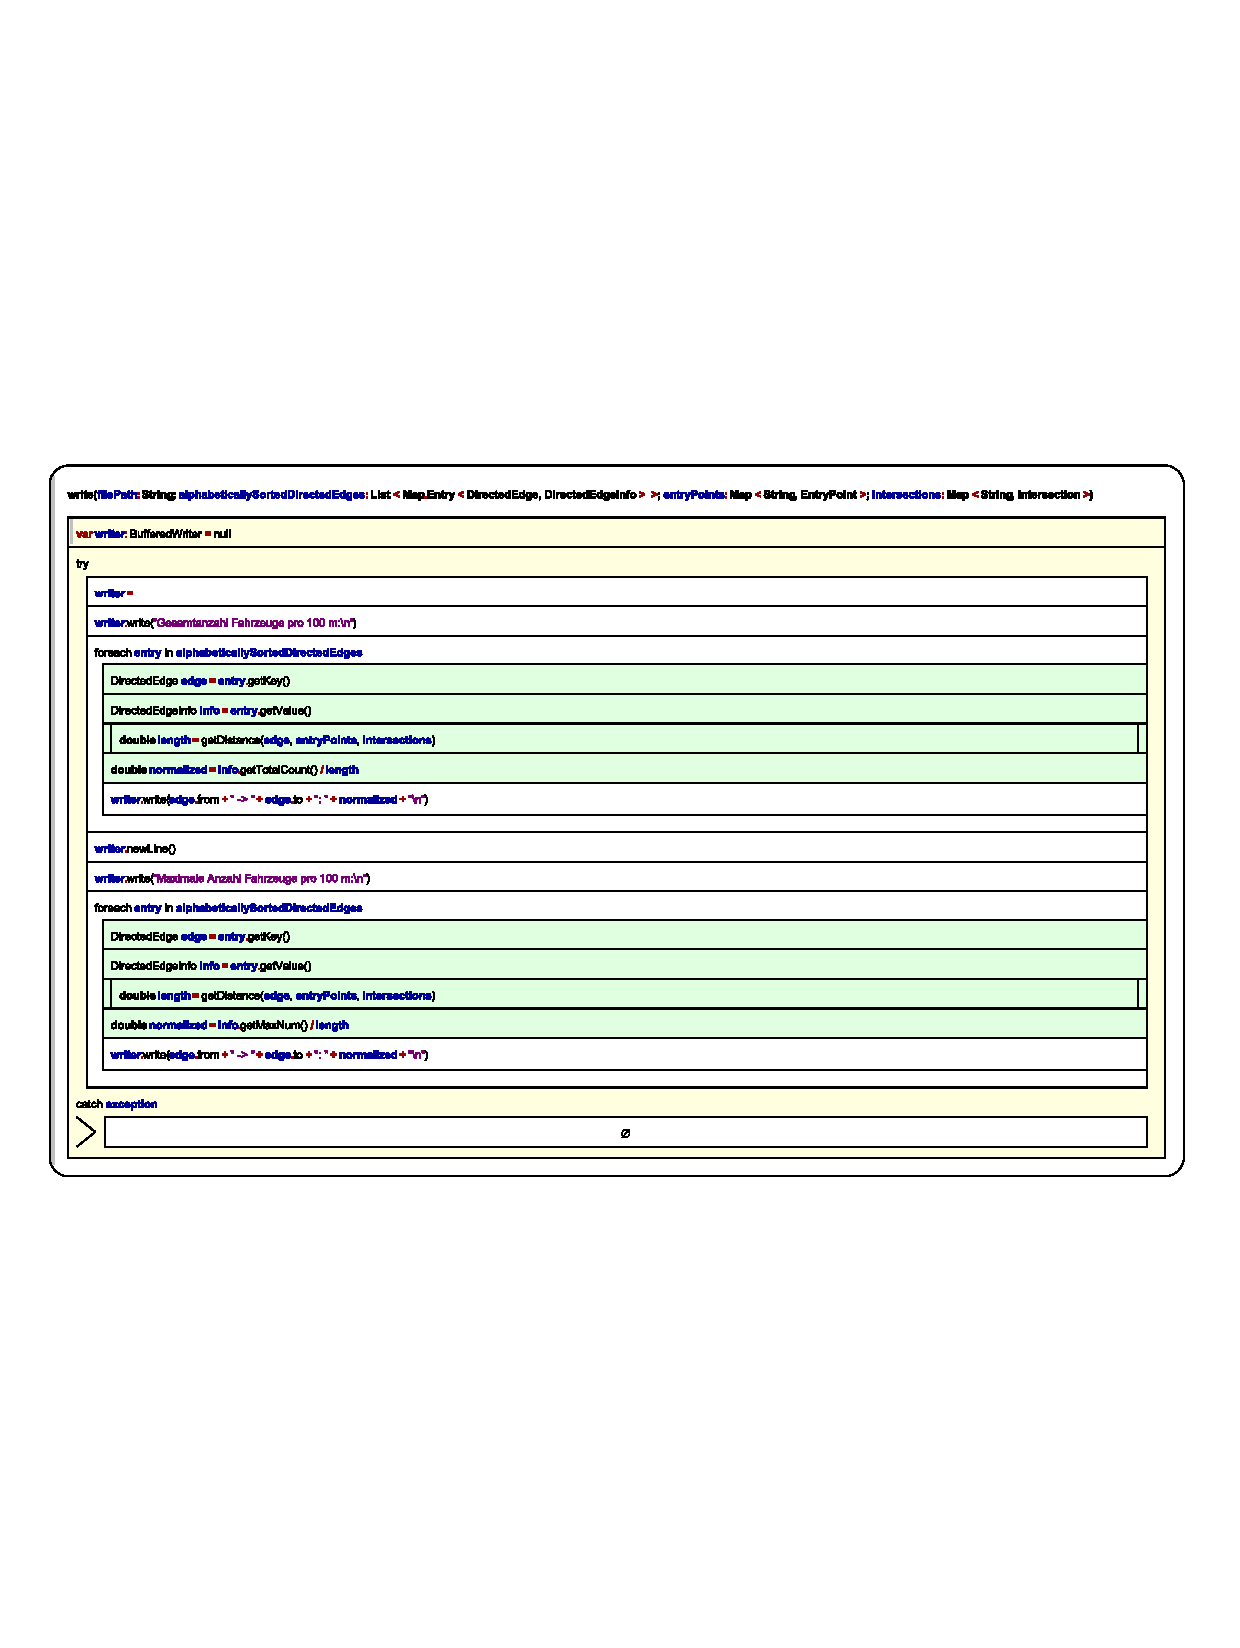
\includegraphics[width=1.05\textwidth]{nassis/Output/writeStats.pdf}}
\end{figure}

\clearpage

  \item \textbf{\texttt{Fahrzeuge.txt} (Klasse \texttt{VehicleWriter})} \\
  Diese Datei protokolliert die Positionen aller Fahrzeuge zu bestimmten Zeitpunkten der Simulation (gesteuert durch den Parameter \texttt{clockRate}). Jeder Zeitstempel ist mit \texttt{*** t = <Sekunden>} markiert. Darunter folgen Zeilen mit:
  \begin{center}
    \texttt{<x\_pos> <y\_pos> <x\_ziel> <y\_ziel> <ID>}
  \end{center}
  Dadurch kann der zeitliche Verlauf der Fahrzeugbewegungen nachvollzogen werden. Die Daten stammen aus der \texttt{vehicleHistory}.
\end{itemize}

\FloatBarrier
        \vspace{-2cm} 
\begin{figure}[h!]
            \vspace{-2cm} 
    \centering
    \makebox[\textwidth][c]{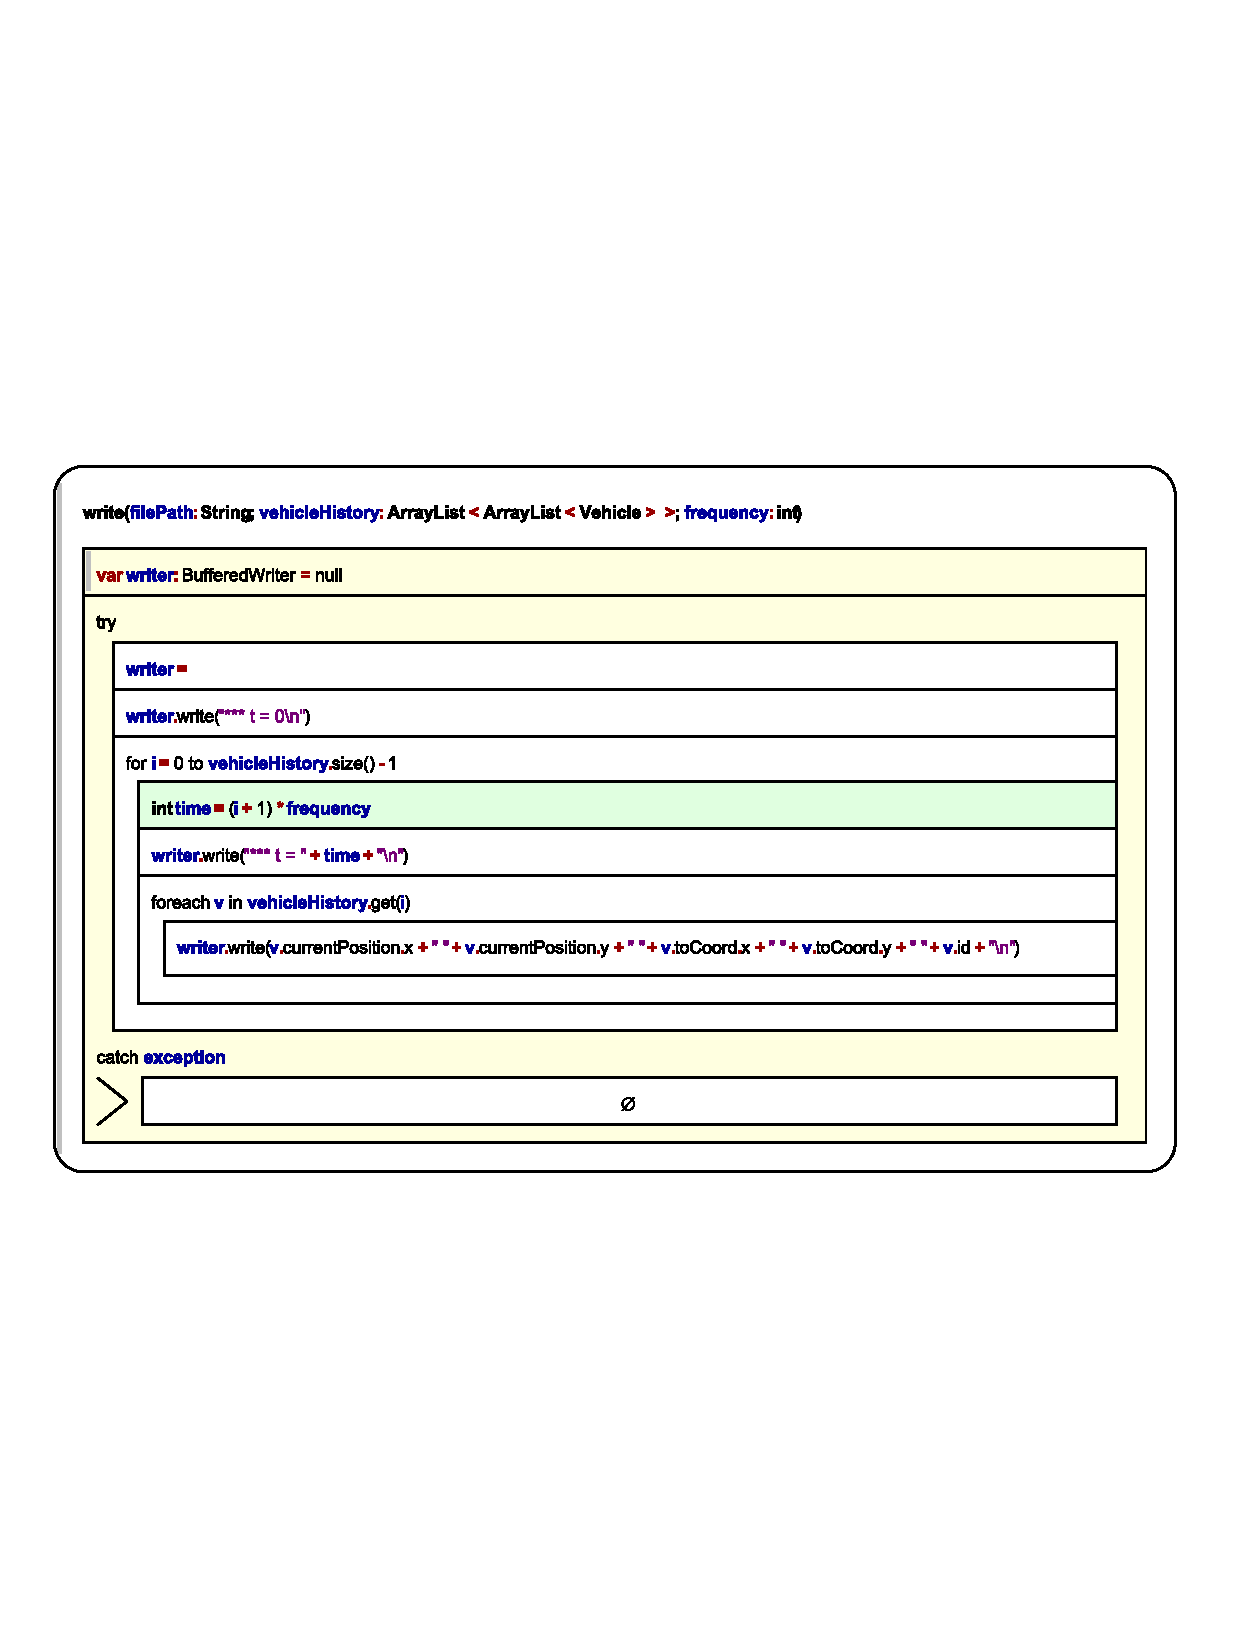
\includegraphics[width=1.05\textwidth]{nassis/Output/writeVehicles.pdf}}
\end{figure}
\FloatBarrier
\vspace{-2cm}
\begin{figure}[h!]
    \vspace{-2cm}
    \centering
    \caption{Klassenstruktur der Ausgabeklassen}
    \makebox[\textwidth][c]{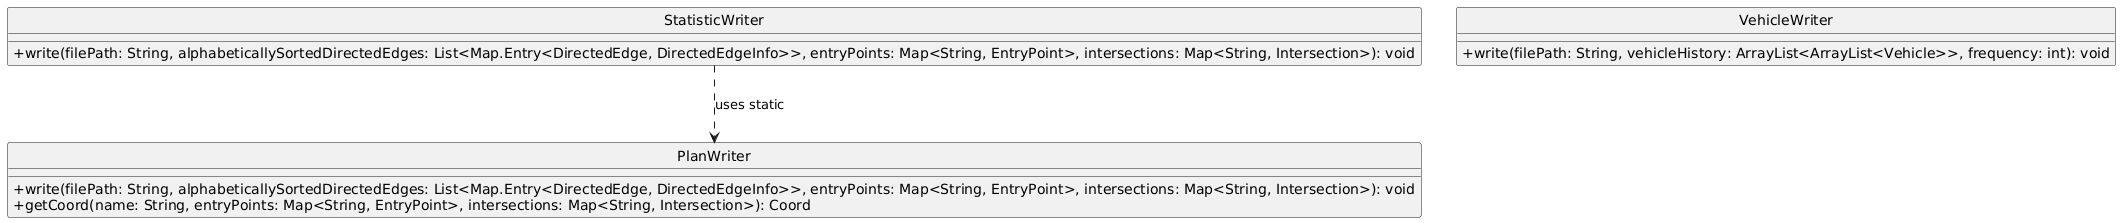
\includegraphics[width=1.05\textwidth]{umlClassDiagrams/outputUml.png}}
\end{figure}


\clearpage

\section{Gesamtablauf}

\begin{enumerate}
  \item \textbf{Programmstart (\texttt{Main.main})}
  \begin{itemize}
    \item Prüfung, ob ein gültiger Dateipfad als Argument übergeben wurde.
    \item Instanziierung eines \texttt{Reader}-Objekts vom Typ \texttt{TextFileReader}.
  \end{itemize}

  \item \textbf{Einlesen der Stadtstruktur (\texttt{reader.read()})}
  \begin{itemize}
    \item Datei wird zeilenweise eingelesen und in Abschnitte gegliedert:
    \begin{itemize}
      \item \texttt{Zeitraum:} Einlesen von \texttt{maxTime} und \texttt{clockRate}.
      \item \texttt{Einfallspunkte:} Aufbau einer Map von Namen auf \texttt{EntryPoint}-Objekte.
      \item \texttt{Kreuzungen:} Aufbau einer Map von Namen auf \texttt{Intersection}-Objekte sowie gerichteter Kanten mit zugehörigem \texttt{DirectedEdgeInfo}.
    \end{itemize}
    \item Durchführung mehrerer Validierungen (z.\,B. doppelte Namen, unerlaubte Referenzen, Mindestabstand von Koordinaten).
    \item Rückgabe eines \texttt{CityDTO}-Objekts.
  \end{itemize}

  \item \textbf{Initialisierung der Simulation (\texttt{new City(CityDTO)})}
  \begin{itemize}
    \item Übernahme aller Eingabedaten in das \texttt{City}-Objekt.
  \end{itemize}

  \item \textbf{Simulationsablauf (\texttt{city.simulate()})}
  \begin{itemize}
    \item Für jede Zeiteinheit $t$ von $1$ bis \texttt{maxTime}:
    \begin{itemize}
      \item \texttt{updateVehicles()}: Bewegung aller Fahrzeuge entlang ihrer aktuellen Kante. Bei Zielerreichung Auswahl eines neuen Ziels oder Entfernen des Fahrzeugs.
      \item Fahrzeugerzeugung an jedem Einfallspunkt, sofern $t \mod \texttt{freq} = 0$.
      \item \texttt{updateDirectedEdgesMaxima()}: Aktualisierung der Maximalwerte pro Kante.
      \item Speicherung eines Snapshots der Fahrzeugzustände in \texttt{vehicleHistory}, wenn $t \mod \texttt{clockRate} = 0$.
    \end{itemize}
  \end{itemize}

  \item \textbf{Erzeugung der Ausgabedateien}
  \begin{itemize}
    \item \texttt{PlanWriter.write}: Ausgabe aller Straßenverbindungen (Koordinatenpaare) in \texttt{Plan.txt}.
    \item \texttt{StatisticWriter.write}: Ausgabe von Nutzungsstatistiken (gesamt / maximal pro 100\,m) in \texttt{Statistik.txt}.
    \item \texttt{VehicleWriter.write}: Ausgabe aller Fahrzeugpositionen zu gespeicherten Zeitpunkten in \texttt{Fahrzeuge.txt}.
  \end{itemize}
\end{enumerate}

\begin{figure}[h!]
    \centering
    \caption{Hauptablauf der Simulation}
    \makebox[\textwidth][c]{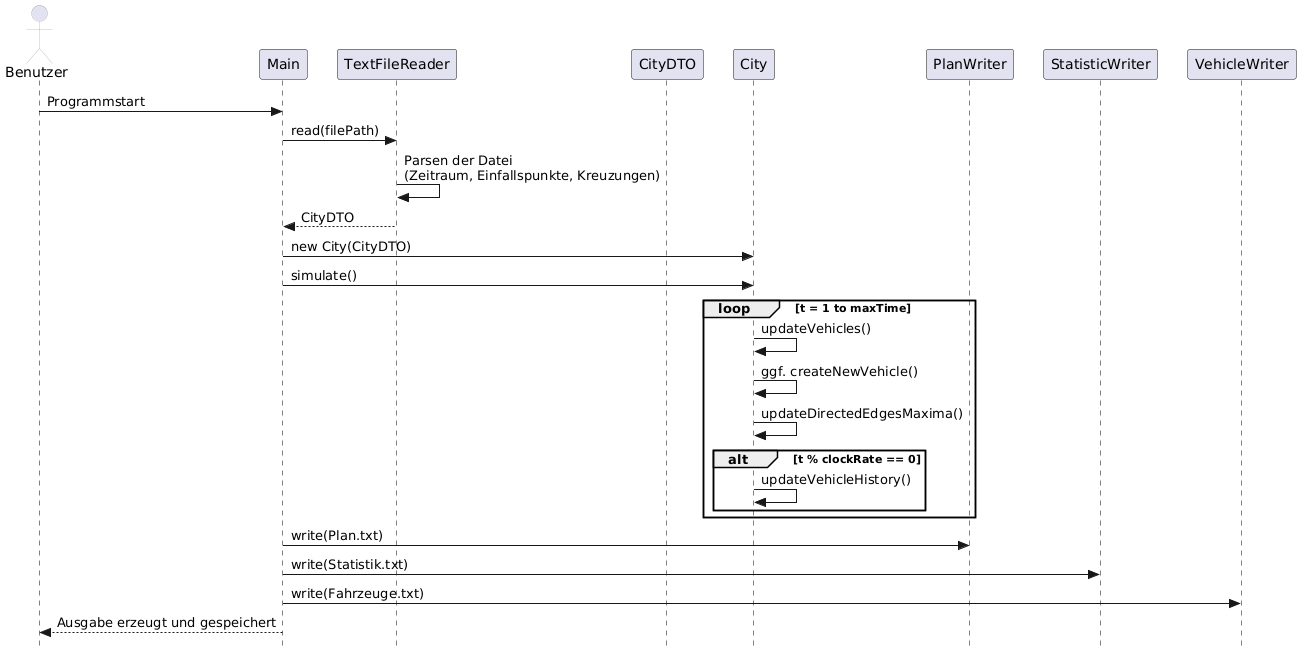
\includegraphics[width=1.3\textwidth]{umlClassDiagrams/MainSequenceDiagram.png}}
\end{figure}



